The HDF5\_BLS\_GUI is a graphical user interface for the HDF5\_BLS package, designed to facilitate the exploration and analysis of HDF5 files. It provides a user-friendly environment for users to interact with their data, visualize results, and manage their workflows.

The GUI is built using the PySide6 library, which is a Python binding for the Qt framework. This library allows the GUI to be developed using a similar syntax to traditional Python code, making it easier to understand and maintain.

The GUI opens to the following window:
\begin{figure}[H]
    \centering
    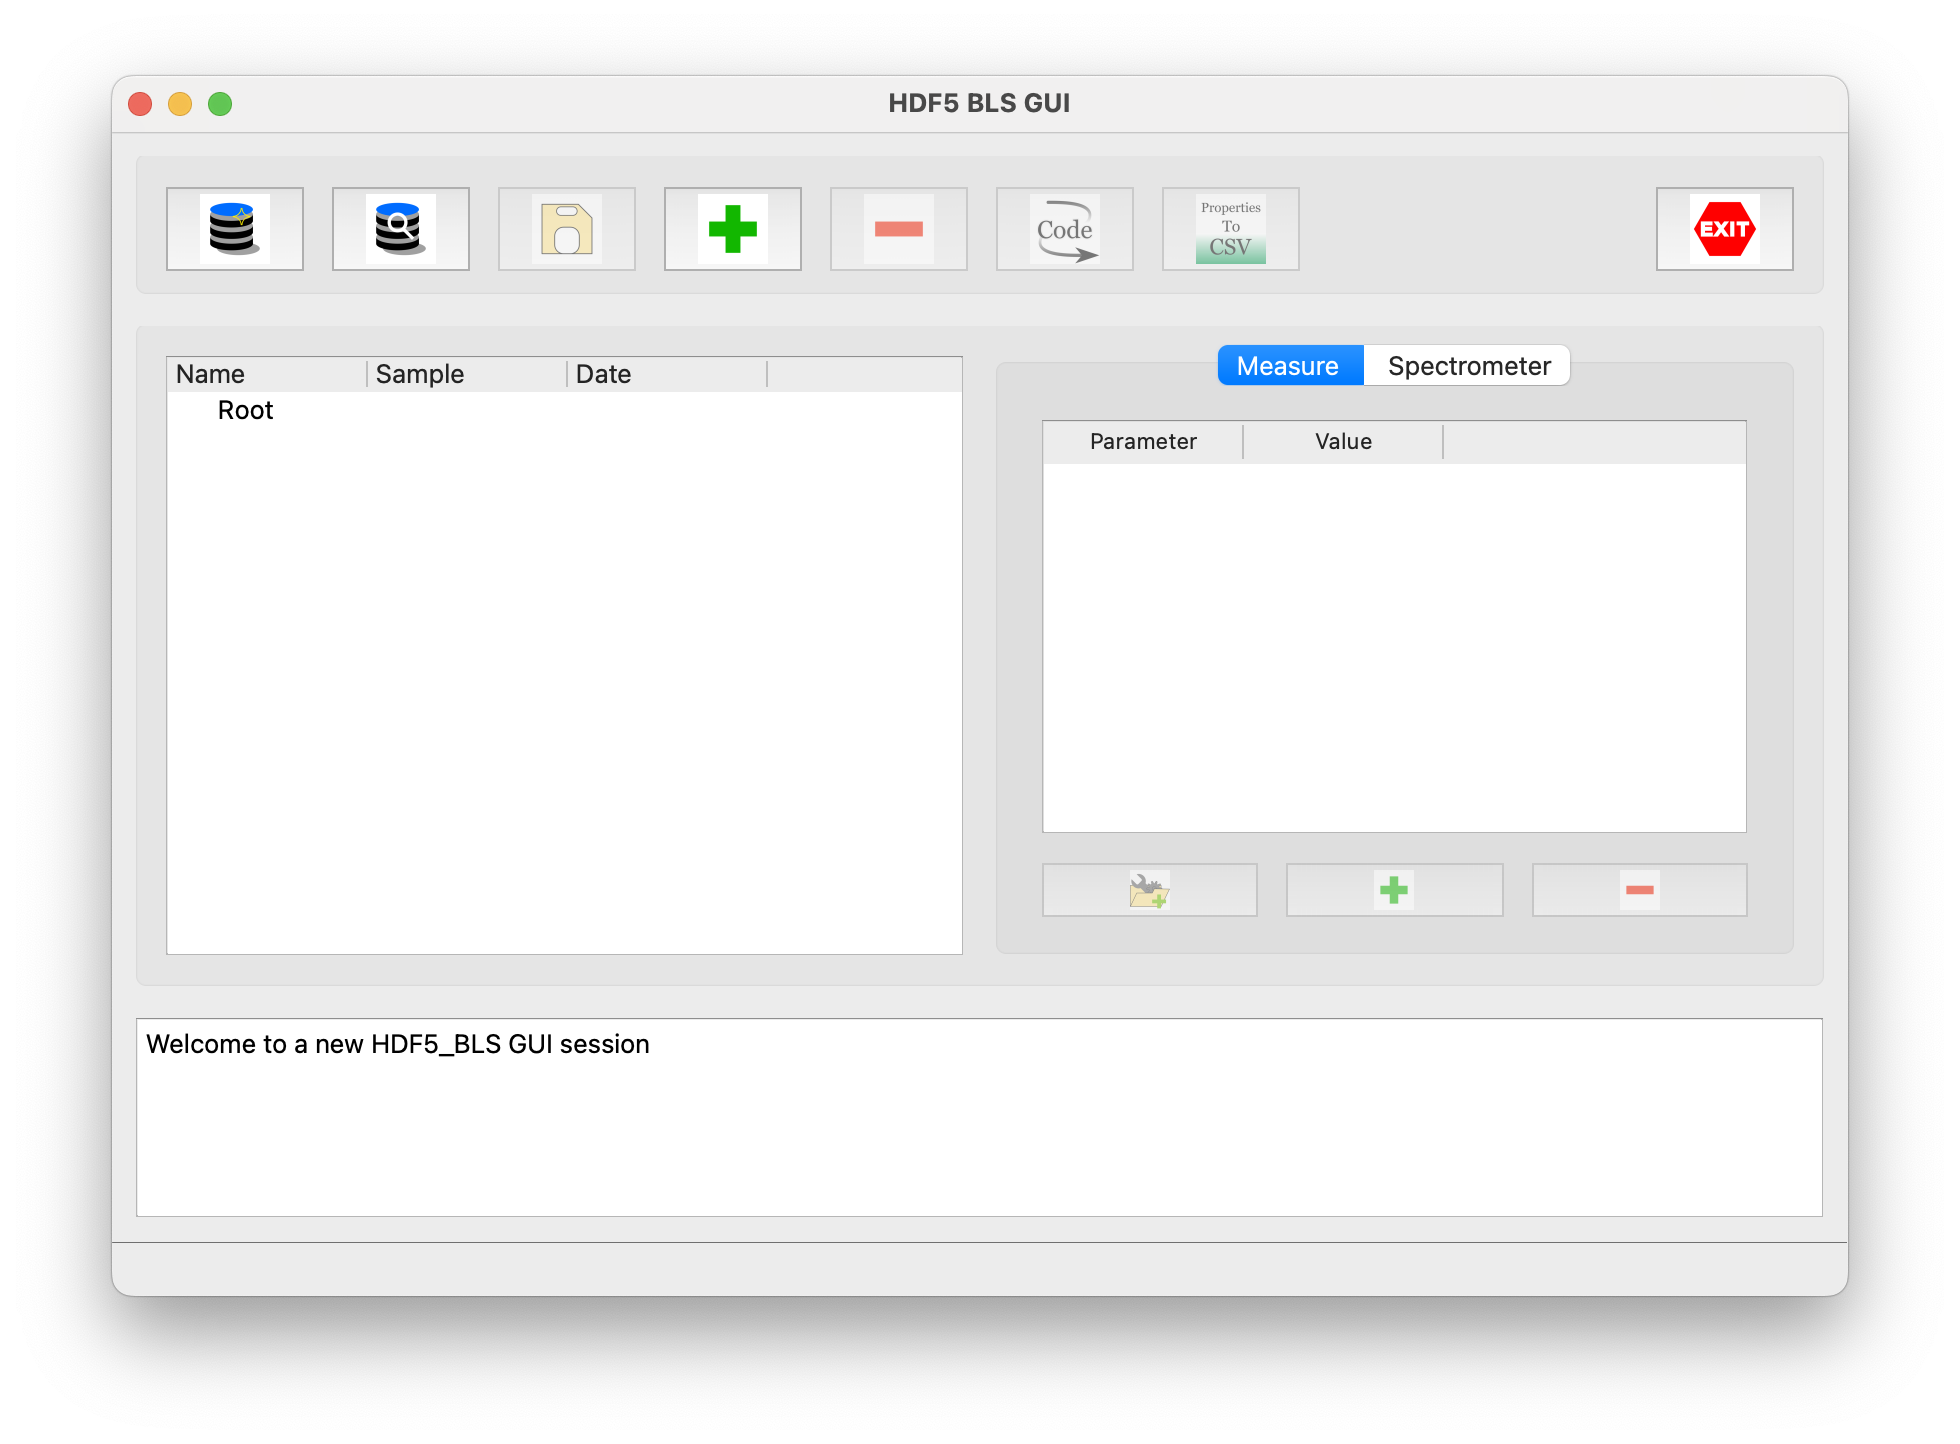
\includegraphics[width=\textwidth]{img/main_window.png}
    \caption{HDF5\_BLS\_GUI Main Window}
    \label{fig:gui_main_window}
\end{figure}

The window is divided into four main sections:
\begin{itemize}
    \item Top: Contains a series of buttons to perform actions on the HDF5 file. The buttons are divided into three categories.
    \item Left: Displays the hierarchical structure of the HDF5 file, allowing users to navigate through its contents.
    \item Right: Shows the properties and metadata of the selected HDF5 object, providing detailed information to the user.
    \item Bottom: Contains a logging area to display messages and information about the current operations.
\end{itemize}

The GUI also comes with left and right clicks capabilities. Left clicking on any item in the hierarchical structure will display its properties in the right panel, while right clicking will open a context menu with additional options. A double click on any of the properties of the right pannel will allow us to edit the property.

The GUI finally comes with a menu where all the properties are recapitulated as well as a few other options.